%\documentclass[sigconf]{acmart}
\documentclass[sigconf, anonymous]{acmart}

\usepackage{booktabs} % For formal tables


% Copyright
%\setcopyright{none}
%\setcopyright{acmcopyright}
%\setcopyright{acmlicensed}
%\setcopyright{rightsretained}
%\setcopyright{usgov}
%\setcopyright{usgovmixed}
%\setcopyright{cagov}
%\setcopyright{cagovmixed}


\usepackage{graphicx}
\usepackage{latexsym}
\usepackage{amsmath}
\usepackage{float}
\usepackage{xspace}
\usepackage{algorithm}
\usepackage{algorithmic}
\usepackage{algorithmwh}
\usepackage{amssymb}
\usepackage{subfigure}
\usepackage{url}
\usepackage[mathscr]{eucal}

\renewcommand{\algorithmicrequire}{\textbf{Input:}}
\renewcommand{\algorithmicensure}{\textbf{Output:}}

\newboolean{showcomments}
%
\setboolean{showcomments}{true}
\ifthenelse{\boolean{showcomments}}
{\newcommand{\nb}[2]{
\fbox{\bfseries\sffamily\scriptsize#1}
{\sf\small$\blacktriangleright$\textit{#2}$\blacktriangleleft$}
}
}
{\newcommand{\nb}[2]{}
}
\newcommand\amin[1]{\nb{Amin}{#1}}
\newcommand\ebrahim[1]{\nb{Ebrahim}{#1}}


%\newtheorem{remark}{Remark}
%\newtheorem{theorem}{Theorem}
%\newtheorem{lemma}{Lemma}
%\newtheorem{proposition}{Proposition}
%\newtheorem{corollary}{Corollary}
%\newtheorem{definition}{Definition}
%
%\newdef{example}{Example}

\usepackage{mathtools}
%\DeclareMathOperator*{\argmax}{argmax}
\DeclareMathOperator*{\argmin}{argmin}
\DeclarePairedDelimiter{\norm}{\lVert}{\rVert}

\newcommand{\head}[1]{\par\smallskip\noindent\textbf{#1}}



% DOI
\acmDOI{10.475/123_4}

% ISBN
\acmISBN{123-4567-24-567/08/06}

%Conference
%\acmConference[WOODSTOCK'97]{ACM Woodstock conference}{July 1997}{El
%  Paso, Texas USA}
%\acmYear{1997}
%\copyrightyear{2016}
%\acmArticle{4}
%\acmPrice{15.00}

% These commands are optional
%\acmBooktitle{Transactions of the ACM Woodstock conference}
%\editor{Jennifer B. Sartor}
%\editor{Theo D'Hondt}
%\editor{Wolfgang De Meuter}


\begin{document}

\title{Relationship Prediction in Dynamic Heterogeneous Information Networks}

%\titlenote{Produces the permission block, and copyright information}
%\subtitle{Extended Abstract}
%\subtitlenote{The full version of the author's guide is available as
%  \texttt{acmart.pdf} document}


\author{Amin Milani Fard}
\affiliation{%
      \affaddr{Department of Computer Science}\\
       \affaddr{New York Institute of Technology}\\
       \affaddr{Vancouver, BC, Canada}\\
}
\email{amilanif@nyit.edu}

\author{Ebrahim Bagheri}
\affiliation{
      \affaddr{Department of Electrical
\& Computer Engineering}\\
       \affaddr{Ryerson University}\\
       \affaddr{Toronto, ON, Canada}\\
}
\email{bagheri@ryerson.ca}

\author{Ke Wang}
\affiliation{
      \affaddr{School of Computing Science}\\
       \affaddr{Simon Fraser University}\\
       \affaddr{Burnaby, BC, Canada}\\
}
\email{wangk@cs.sfu.ca}

%\author{Philip S. Yu}
%\affiliation{
%      \affaddr{Dept. of Computer Science}\\
%       \affaddr{University of Illinois at Chicago}\\
%       \affaddr{Chicago, Illinois, USA}\\
%}
%\email{psyu@cs.uic.edu}


% The default list of authors is too long for headers.
\renewcommand{\shortauthors}{A. Milani Fard et al.}


\begin{abstract}

Most real-world information networks, such as social networks, are heterogeneous and as such, the relationships observed in these networks can be diverse and carry differing semantics.
 %relations between different entities have different semantic meanings. 
 Therefore techniques for link prediction in homogeneous networks cannot be directly applied on heterogeneous ones. On the other hand, works that investigate link prediction in heterogeneous networks do not necessarily consider network dynamism in sequential time intervals. In this work we propose a technique that leverages a combination of latent and topological meta path-based features to predict a target relationship between two nodes of given types in a dynamic heterogeneous information network. \ebrahim{Before saying "in our experiments" we need to enumerate the distinguishing aspects of our work and say why they are significant contributions.}Our experiment results on two real-world information network datasets show 10-40\% increase in AUCROC, and 25-30\% increase in prediction accuracy compared to the state of the art techniques.
 
%\keywords{Link prediction \and Relationship prediction \and Dynamic heterogeneous networks \and Social networks \and Network topology \and Meta path.}

\end{abstract}


%
% The code below should be generated by the tool at
% http://dl.acm.org/ccs.cfm
% Please copy and paste the code instead of the example below.
%
%\begin{CCSXML}
%<ccs2012>
% <concept>
%  <concept_id>10010520.10010553.10010562</concept_id>
%  <concept_desc>Computer systems organization~Embedded systems</concept_desc>
%  <concept_significance>500</concept_significance>
% </concept>
% <concept>
%  <concept_id>10010520.10010575.10010755</concept_id>
%  <concept_desc>Computer systems organization~Redundancy</concept_desc>
%  <concept_significance>300</concept_significance>
% </concept>
% <concept>
%  <concept_id>10010520.10010553.10010554</concept_id>
%  <concept_desc>Computer systems organization~Robotics</concept_desc>
%  <concept_significance>100</concept_significance>
% </concept>
% <concept>
%  <concept_id>10003033.10003083.10003095</concept_id>
%  <concept_desc>Networks~Network reliability</concept_desc>
%  <concept_significance>100</concept_significance>
% </concept>
%</ccs2012>
%\end{CCSXML}
%
%\ccsdesc[500]{Computer systems organization~Embedded systems}
%\ccsdesc[300]{Computer systems organization~Redundancy}
%\ccsdesc{Computer systems organization~Robotics}
%\ccsdesc[100]{Networks~Network reliability}


\keywords{Link prediction, relationship prediction, dynamic heterogeneous networks, social networks, network topology, meta path.}


\maketitle

\section{Introduction}
\label{Sec:Introduction}

% what is link prediction problem? what is the usages of link prediction?
% challenges in heterogeneous link prediction, what is not covered? temporal and hero?

The goal of link prediction in a network \cite{liben2007link} is to estimate the likelihood of a future relationship between two nodes based on the observed graph. Predicting such connections in a network %have multiple applications 
can be applied in different contexts such as recommendation systems 
\cite{chen2005link,song2009scalable,lu2012recommender,li2013recommendation,guy2015social}, network reconstruction \cite{guimera2009missing}, node classification \cite{gallagher2008using}, or biomedical applications such as predicting protein-protein interactions \cite{lei2012novel}. Traditional link prediction techniques, such as \cite{liben2007link}, consider networks to be homogeneous, i.e., graphs with only one type of nodes and edges. However, most real-world networks, such as social networks, scholar networks, patient networks \cite{denny2012mining} and knowledge graphs \cite{wang2015incorporating} are heterogeneous information networks (HINs) \cite{shi2017survey} and have multiple node and relation types. For example, in a bibliographic network, there are nodes of types authors, papers, and venues, and edges of types writes, cites and publishes.

In a HIN, relations between different entities carry different semantics. For instance the relationship between two authors are different in meaning when they are co-authors compared to the case when one cites another's paper. Thus techniques for homogeneous networks \cite{liben2007link,wang2007local,lichtenwalter2010new,leroy2010cold,al2006link} cannot be directly applied on heterogeneous ones. A few works such as \cite{sun2011ASONAM,Sun:2012:HRP:2124295.2124373} investigated the problem of link prediction in HINs, however, they do not consider the dynamism of networks and overlook the potential benefits of analyzing a heterogeneous graph as a sequence of network snapshots. To this end, existing work has already shown that in homogenous networks incorporating temporal changes improves link prediction accuracy \cite{Zhu2016}. Previous work on temporal link prediction scarcely studied HINs and to the best of our knowledge, the problem of predicting relationships in dynamic heterogeneous networks has not been studied before. A dynamic heterogeneous information network (DHIN) is a HIN, whose links have associated timestamps.

In this work we study the problem of relationship prediction in a DHIN, which can be stated as: \textit{Given a DHIN graph $G$ at $t$ consecutive time intervals, the objective is to predict the existence of a particular relationship between two given nodes at time $t+1$.} The major challenge in relationship prediction in DHINs is how to effectively combine the HIN topology features and inferred latent features that incorporate temporal changes in order to exhibit the best performance. Also, the prediction technique should be computationally efficient for large-scale networks. To this end, the main contributions of our work include:


%\textit{Given a DHIN graph $G$ at time $t$, how can we predict the existence of a particular relationship/path between two given nodes at time $t+1$?"}


%\cite{Zhu2016} \cite{sun2011pathsim} \cite{Sun:2012:HRP:2124295.2124373}  \cite{huang2016meta} \cite{wang2016relsim} \cite{sun2013pathselclus} \cite{sun2011ASONAM} \cite{Yang2012} \cite{liben2007link}


%\subsection{Motivation}
% what are the challenges in directly applying the current techniques?
% To address the above challenges, we propose a new ... First, , we introduce the concept of augmented graph, which allows us to incorporate more complex semantics into our prediction problem. Second, instead of computing the ...., we use all of the latent features of all meta-graphs. ...


%In \cite{gu2018rare} authors presented SocialRank...


%The main objective of this work is to examine possibility of using meta path-based features along with latent features ... To this end, we propose to ... by taking into account (i) theory of Homophily [12], which refers to the tendency of users to connect to users with common interests or preferences; and (iii) relationship between emerging topics, based on their similar constituent contents and user contributions towards them. More specifically, the key contributions of our work are as follows:


\begin{itemize}

\item We propose the problem of relationship prediction in a DHIN, and draw a contrast between this problem and existing link prediction techniques that have been proposed for dynamic and heterogeneous networks;

\item We present a simple yet effective technique, called \textit{MetaDynaMix}, that leverages topological meta path-based and latent features to predict a target relationship between two nodes in a DHIN;

%\item We define the \textit{augmented reduced graph} that is generated according to a given HIN and a target relation meta path and is used in our proposed algorithms: the homogenize link prediction, and the dynamic meta path-based relationship prediction;

%\item We implement our approach in a tool called ..., which is freely available

\item We empirically evaluate the accuracy of our proposed work on two real-world datasets, and the results show 10-40\% increase in AUCROC, and 25-30\% increase in prediction accuracy compared to the state of the art baselines.

\end{itemize}


%In the rest of the paper, we introduce the preliminaries and problem statement in Section 2, discuss our solutions to the relationship prediction problem in Section 3, explain the details of our empirical experimentation and findings in Section 4, review the related work in Section 5, and finally conclude the paper.

\section{Problem Statement}

\begin{definition}[Dynamic heterogeneous social network]
A dynamic heterogeneous social network is defined as a directed graph $G$ = ($V$, $E$), where $V$ and $E$ are set of nodes and edges of different types, and edges have timestamps. $\Box$
\end{definition}

\begin{example}
The DBLP bibliographic network\footnote{\url{http://dblp.uni-trier.de/db/}} is a dynamic heterogeneous social network, containing different types of nodes such as papers, authors, topics, and publication venues, with publication links associated with date. Twitter social network is another example with nodes of types posted tweets, users, topics, and hashtags and time window associated with these tweets. $\Box$
\end{example}

In the context of a heterogenous network, a \textit{link} can be either \textit{direct} or \textit{indirect}. An indirect link is a sequence of relationships (direct links) in the network. Thus, two nodes might not be directly connected, however they might be connected considering the semantic of a sequence of links of different types. In this work, therefore, the \textit{link prediction} problem refers to predicting whether two nodes will be connected in future via a sequence of relationships in the graph. Note that the length of sequence can be greater than or equal to one. For instance in a bibliographic network a direct link exist between an author and a paper he wrote, and an indirect link exist between him and his co-authors through the paper, which they wrote together.

\begin{definition}[\textbf{Link prediction problem}]\label{problemdef}
 Given A dynamic heterogeneous social network $G$ at time $t$ and a target relation $R$, we aim to predict a link of type $R$ between two given nodes at time $t+1$. $\Box$
 \end{definition}

In order to better understand different types of nodes and their relation in a network, the concept of \textit{network schema} \cite{sun2011pathsim} is used. The network schema is a meta structure graph that summarizes a heterogeneous social network and is formally defined as bellow.

\begin{definition}[Network schema]
The network schema $S_G=\mathcal{(A,R)}$ is a directed meta graph for a heterogeneous network $G=(V,E)$, where $\mathcal{A}$ is the set of node types in $V$ and $\mathcal{R}$ is the set of relation types in $E$.  $\Box$
\end{definition}

\begin{example}
Figure \ref{schema} shows the network schema for DBLP bibliographic network, where $\mathcal{A}$=\{\textit{Authors}, \textit{Paper}, \textit{Venues}, \textit{Topics}\}. $\Box$
\end{example}

In this paper, we refer to different types of nodes for DBLP bibliographic network using abbreviations $P$ for papers, $A$ for authors, $T$ for topic, and $V$ for venues. 

\begin{figure}[t]
  \centering
      \includegraphics[width=0.4\textwidth]{figs/schema.pdf}
  \caption{Network schema for DBLP network.}\label{schema}
\end{figure}

\subsection{Meta path-based topology}

Similar to the notion of network schema that provides a meta structure for the network, a \textit{meta path} \cite{sun2011pathsim} provides a meta structure for paths between different nodes in the network. 

\begin{definition}[Meta path]
A meta path $\mathcal{P}$ is a path in the network schema graph $S_G = (\mathcal{A,R})$, denoted in the form of $\mathcal{P} = A_1 \xrightarrow{R_1} A1... \xrightarrow{R_n} A_{n+1}$, as a sequence of relations between node types, which defines a new composite relation between its starting type and ending type. $\Box$
\end{definition}



\begin{example}
In the DBLP network example, the co-author relation can be described with the meta path $A\xrightarrow{write}P\xrightarrow{write^{-1}}A$ or in short form \textit{A--P--A}. Paths in thick solid lines in Figure \ref{sampleNetwork} correspond to \textit{A--P--V--P--A} meta paths between Max and Ada. $\Box$

\end{example}

Each meta path indicates a different semantic for a path connecting two nodes, and defines a unique topology representing a special relation.

\begin{figure}[t]
  \centering
      \includegraphics[width=0.4\textwidth]{figs/exampleSocialNetwork.pdf}
  \caption{An example of \textit{A--P--V--P--A} meta paths between two authors Max and Ada.}\label{sampleNetwork}
\end{figure}



%By checking the existing topological features defined in homogeneous networks, we can find that both the neighbor set-based features and path-based features can be generalized in heterogeneous information networks, by considering paths following different meta paths. For example, if we treat each type of neighbors separately and extend the immediate neighbors to n-hop neighbors (i.e., the distance between one object and its neighbors are n), the common neighbor feature between two authors is then becoming the count of paths between the two authors following different meta paths. For path-based features, such as Katz, it can be extended as a combination of paths following different meta paths. 



\section{Relationship Prediction Approach}

Given a DHIN graph $G=(V,E)$, and the number of graph snapshots $t$, we first decompose $G$ to a sequence of $t$ HIN graphs ${G_1, .., G_t}$ based on links with associated timestamps. We then apply our techniques to predict $G_{t+1}$. As mentioned in Definition \ref{problemdef}, in this work we intend to predict \textit{existence of a given type of relationship} (target meta path) between two given nodes. Therefore we define a new type of graph, called \textit{augmented reduced graph}, that is generated based on a given heterogeneous graph and a target relation meta path. 

\begin{definition}[Augmented reduced graph]\label{def:ARG}
Given a HIN graph $G=(V,E)$ and a target meta path $P(A_i,A_j)$ between nodes of type $A_i$ and $A_j$, an \textit{augmented reduced graph} $G^P=(V^P,E^P)$ is a graph, where $V^P \subseteq V$ and nodes in $V^P$ are of type $A_i$ and $A_j$, and edges in $E^P$ indicates relationships of type $P$ in $G$. $\Box$
\end{definition}

%\begin{example}
An augmented reduced graph for the network in Figure \ref{sampleNetwork} and target meta path $P(A,A)$=\textit{A--P--V--P--A} is a graph with nodes of type \textit{Author} and edges that represent relationship of \textit{publishing in the same venue}. For example (\textit{Max}, \textit{Ada}) is an edge in the corresponding augmented reduced graph because they both published at KDD and ICDM. If we consider meta path $P(A,A)$=\textit{A--P--A}, the augmented reduced graph represents a co-authorship graph, where nodes are of type \textit{Author} and edges, such as (\textit{Max}, \textit{Tom}), represent \textit{co-authorship}.  
%$\Box$
%\end{example}


%\subsection{Algorithm}

\subsection{Homogenize link prediction}
% We refer to this approach as \texttt{HomoTemp}.

Zhu et al. \cite{Zhu2016} studied the problem of temporal link prediction in the context of homogeneous networks, where the input is a sequence of graphs $G_1, ..., G_t$ and the output is the estimated $G_{t+1}$. The authors presented a matrix factorization (MF) with block-coordinate gradient descent technique that for each $G_\tau$ at time $\tau$ infers a low rank $k$-dimensional latent space representation matrix $Z_\tau$ that minimizes the quadratic loss with temporal regularization
\begin{equation}\label{latentOrigEqu}
    \begin{array}{l}
\argmin\limits_{Z_1, .., Z_t}\sum\limits_{\tau=1}^{t}\left \| G_\tau-Z_{\tau}Z_{\tau}^T \right \|^2_F+\lambda \sum\limits_{\tau=1}^{t}\sum\limits_{u}(1-Z_{\tau}(u)Z_{\tau-1}(u)^T) 
\\
\text{subject to :} \forall u,\tau,Z_{\tau}\geq 0, Z_{\tau}(u)Z_{\tau}(u)^T=1
    \end{array}
\end{equation}
where $\lambda$ is a regularization parameter, and  $(1-Z_{\tau}(u)Z_{\tau-1}(u)^T)$ penalizes node $u$ for suddenly changing its latent position. %Note that when computing the quadratic loss $\left \| G^R_\tau-Z_{\tau}BZ_{\tau}^T \right \|^2_F$, we ignore all of the diagonal entries.
$Z_\tau(u)$ is a row vector denoting $u$'s temporal latent space representation at time $\tau$, and $Z_\tau(u,i)$ indicates the position of $u$ in the $i$-th dimension at $Z$. The intuition behind their prediction model is that 1) nodes move smoothly in the latent space over time and it is less likely to have large moves \cite{sarkar2005dynamic,zhang2014inferring}, and 2) user interactions are more likely to occur between similar users in a latent space representation. The authors used $Z_tZ_t^T$ to predict $G_{t+1}$ in their work, however, they mentioned that $G_{t+1}$ can be formulated as $\Phi(f(Z_1,...Z_t))$, where $\Phi$ is the link function and $f$ is the temporal function and one may apply techniques such as nonparametric approaches \cite{Sarkar:2012} to automatically learn these functions.

An immediate adaptation of the above MF technique is to consider a sequence of augmented reduced graphs $G^P_i$ as input, i.e., graphs with source and destination of a target meta path with edges between them if the target meta path exists in $G_i$. This changes equation (\ref{latentOrigEqu}) by replacing $G_\tau$ with $G^{P}_\tau$.


%to the following
%\begin{equation}\label{latentReducedEqu}
%    \begin{array}{l}
%\argmin\limits_{Z_1, .., Z_t}\sum\limits_{\tau=1}^{t}\left \| G^{P}_\tau-Z_{\tau}Z_{\tau}^T \right \|^2_F+\lambda \sum\limits_{\tau=1}^{t}\sum\limits_{u}(1-Z_{\tau}(u)Z_{\tau-1}(u)^T) 
%\\
%\text{subject to :} \forall u,\tau,Z_{\tau}\geq 0, Z_{\tau}(u)Z_{\tau}(u)^T=1
%    \end{array}
%\end{equation}

%Their MF technique \cite{Zhu2016} to infer $Z_t$ and estimate $G_{t+1}^R$. We refer to this approach as \texttt{HomoTemp}.


Algorithm \ref{alg1} gets as an input a DHIN graph $G$, number of graph snapshots $t$, a target relation meta path $P(a,b)$, and latent space dimension $k$. The algorithm first decomposes $G$ into a sequence of graphs $\{G_1, .., G_t\}$ (line 1) by considering the associated timestamps on edges. Next from each graph snapshot $G_i$, a corresponding augmented reduced graph $G^P_i$ is generated (lines 2-8) for which nodes are of type $a$ and $b$ (beginning and end of target relation meta path $P$). Finally the MF technique in \cite{Zhu2016} is applied (lines 9-10) to infer $k$-dimensional temporal latent spaces $Z_1, ...,Z_t$ and estimate $G^P_{t+1}$ by $Z_tZ_t^T$.
\amin{How $Z_{t+1}$ depends on $Z_1, ..., Z_t$ from the algorithm? Explain assumptions in \cite{Zhu2016}.}


\begin{algorithm}[t]
\caption{Homogenize Link Prediction}\label{alg1}
\begin{algorithmic}[1]\scriptsize
\REQUIRE A DHIN graph $G$, number of graph snapshots $t$, a target relation meta path $P(a,b)$, latent space dimension $k$
\ENSURE The predicted graph $G^P$ at time $t+1$ based on the given target relation meta path $P$

\STATE $\{G_1, .., G_t\} \leftarrow DecomposeGraph(G, t)$

\FOR {each graph $G_i$}
    %\STATE $G^R_i \leftarrow AugmentedReducedGraph(G_i,P,S)$
    \STATE Let $a$ and $b$ be the node types of beginning and end of $P$
    
    %\FOR {each path $p$ between nodes of type $a$ and $b$ in $S$}
    \FOR {each node $x \in V_i$ of type $a$ in $G_i$}
        \STATE follow $P$ to reach a node $y$ of type $b$ in $G_i$ 
        \STATE add edge $(x,y)$ to augmented reduced graph $G_i^P$ 
\ENDFOR

\ENDFOR
%\STATE $G^R_{t+1} \leftarrow MF(G^R,k)$ \cite{Zhu2016}
\STATE Infer temporal latent spaces $Z_1, .., Z_t$ using \textit{MF}%by optimizing Eq. \ref{latentReducedEqu}

\STATE $G^P_{t+1} \leftarrow Z_tZ^T_t$ 

\STATE return $G^P_{t+1}$
\end{algorithmic}
\end{algorithm}



\subsection{Meta path-based relationship prediction}

The homogenize approach, however, does not consider different semantics of meta paths between the source and destination nodes. In fact, Zhu et al. \cite{Zhu2016} assume that the probability of a link between nodes depends only on their latent positions. However, we also consider meta path-based features in our prediction model. Our intuition is that leveraging meta path-based features \cite{sun2011pathsim} helps to boost prediction accuracy besides using latent space feature space. In other word, we combine latent space features with topological meta path-based features.

We define a set of meta paths \cite{sun2011pathsim} on a given network schema and a target relation meta path $P$, such as co-authorship, to generate an augmented reduced graph (Definition \ref{def:ARG}) $G^P_i$ from $G_i$ based on $P$.  We then leverage the technique in \cite{Zhu2016} to predict $G^P_{t+1}$ given $G^P_1, ..., G^P_t$, by inferring the temporal latent space representation for nodes at time $t+1$.\amin{this para seems wrong!!!}

Algorithm \ref{alg2} gets as an input a DHIN graph $G$, number of graph snapshots $t$, a network schema $S$, target relation meta path $P(a,b)$ between node types $a$ and $b$, maximum length of a meta path $l$, and latent space dimension $k$. Same as Algorithm \ref{alg1}, it decomposes $G$ into a sequence of graphs (line 1). It then produces the set of all meta paths between a node type $a$ and type $b$ defined in the given target relation $P(a,b)$ (line 2). This is done by traversing the network schema $S$ (for instance through a BFS traversal) and generating meta paths with maximum length of $l$ .

\begin{algorithm}[t]
\caption{Meta path-based Link Prediction}\label{alg2}
\begin{algorithmic}[1]\scriptsize
\REQUIRE A dynamic heterogeneous graph $G$, number of graph snapshots $t$, network schema $S$, a target relation meta path $P^*(a,b)$, maximum length of a meta path $l$, latent space dimension $k$
\ENSURE The predicted graph $G^{P^*}$ at time $t+1$ based on the given target relation $P^*$

\STATE $\{G_1, .., G_t\} \leftarrow DecomposeGraph(G, t)$

\STATE $\{P_1, .., P_n\} \leftarrow GenerateMetaPaths(S, P^*(a,b), l)$

\FOR {each meta path $P_j(a,b)$}

\FOR {each graph $G_i$}
    %\STATE $G^R_i \leftarrow AugmentedReducedGraph(G_i,R,S)$
    %\STATE Let $a$ and $b$ be the node types of beginning and end of $P_j$
    
    %\FOR {each path $p$ between nodes of type $a$ and $b$ in $S$}
    \FOR {each node $x \in V_i$ of type $a$ in $G_i$}
        \STATE follow $P_j$ to reach a node $y$ of type $b$ in $G_i$ 
        \STATE $w_{xy} \leftarrow MeasureSimilarity(x,y, G_i)$
        \STATE add edge $(x,y)$ with weight $w_{xy}$ to augmented reduced graph $G_i^{P_j}$ 
\ENDFOR

\ENDFOR

%\STATE $G^R_{t+1} \leftarrow MF(G^R,k)$ \cite{Zhu2016}
\STATE Infer temporal latent spaces $Z_1, .., Z_t$ using \textit{MF}%by optimizing Eq. \ref{latentReducedEqu}
\STATE $G^{P_j}_{t+1} \leftarrow Z_tZ^T_t$ 

\ENDFOR

\STATE $G^{P^*}_{t} \leftarrow LastKnownTargetGraph(G, P^*(a,b), t)$


\STATE $\forall (a,b\in N(a)) \in G^{P^*}_{t}$, add a feature vector to the training set with $w_{ab}$ in $G^{P_j}_{t-1}$ for each meta paths $P_j$, and label with 1 if $(a,b) \in E^{P^*}_{t}$ otherwise 0.

\STATE Learn the model and apply it to the feature vector of $G^{P_j}_{t+1}$ with different meta path $P_j$.

\STATE Build $G^{P^*}_{t+1}$ based on the cut-off values for the output of prediction model.

\STATE return $G^{P^*}_{t+1}$
\end{algorithmic}
\end{algorithm}


 Next from each graph snapshot $G_i$, a corresponding augmented reduced graph $G^P_i$ is generated (lines 3-9) for which nodes are of type $a$ and $b$ (beginning and end of meta path $P$) and edges have weight between 0 and 1, based on a similarity measure. For example PathCount\cite{sun2011pathsim}, PathSim \cite{sun2011pathsim}, or random walk are measures for the relation of two nodes given link type and meta path, such as co-authorship.
\amin{Note that values of $G^P_i$ depends on meta-path $P$}. Once the sequence of augmented reduced graphs \{$G^P_1, ..., G^P_t$\} are generated, we apply the matrix factorization with the MF technique \cite{Zhu2016} to find a low rank $k$-dimensional latent space representation matrix $Z_\tau$ for nodes at time $\tau$.

% \begin{equation}\label{latentEqu}
%     \begin{array}{l}
% \argmin\limits_{Z_1, .., Z_t}\sum\limits_{\tau=1}^{t}\left \| G^{R_i}_\tau-Z_{\tau}Z_{\tau}^T \right \|^2_F+\lambda \sum\limits_{\tau=1}^{t}\sum\limits_{u}(1-Z_{\tau}(u)Z_{\tau-1}(u)^T) 
% \\
% \text{subject to :} \forall u,\tau,Z_{\tau}\geq 0, Z_{\tau}(u)Z_{\tau}(u)^T=1
%     \end{array}
% \end{equation}




%* Restrict pathSim to 3-hops and not beyond

\subsubsection{The predictive model.} Given the training pairs of nodes and their corresponding meta path-based features (similarity weights $w$), we build a prediction model to learn the weights associated with these features by apply logistic regression. We define the probability of existence of a link between nodes $a$ and $b$ as 
$Pr(label = 1|a, b; \boldsymbol{\theta}) = \frac{e^{z}}{e^{z}+1}$
where $z=\sum\limits_{i=1}^{n}\theta_i.w_i$ for $n$ meta paths, and $\theta_i$ is a normalized weight value for $w_i$ (meta path-based feature). We use logistic regression with $L_2$ regularization to estimate the optimal $\theta$. 
%$\boldsymbol{\hat{\theta}} = 
%\operatorname*{arg\,max}_{\boldsymbol{\theta}}\sum_i log Pr(y_i = 1|a_i, b_i; \boldsymbol{\theta}) - \alpha \sum_{j=1}^N \theta_j^2
%$

\begin{equation*}
\boldsymbol{\hat{\theta}} = 
\operatorname*{arg\,max}_{\boldsymbol{\theta}}\sum_i log Pr(y_i = 1|a_i, b_i; \boldsymbol{\theta}) - \alpha \sum_{j=1}^N \theta_j^2
\end{equation*}

We derive \textbf{$\hat{\theta}$} which maximizes the likelihood of all the training pairs, using maximum likelihood estimation.


In the training phase, for each pair of nodes $(a,b)$ in $G^{P^*}_{t}$, where $b \in N(a)$, we add a feature vector to the training set with corresponding $w_{ab}$ in $G^{P_j}_{t-1}$ for each meta paths $P_j$, and with label 1 if $(a,b) \in E^{P^*}_{t}$ otherwise label 0. We then perform logestic regression to learn the model. Finally we apply the model to the feature vector of predicted graphs $G^{P_j}_{t+1}$ with different meta path $P_j$. Finally it builds $G^{P^*}_{t+1}$ based on the cut-off values for the output of prediction model.


\subsection{Combining latent and meta path-based features}

\amin{ISSUES TO DISCUSS}

Zhu et al. \cite{Zhu2016} studied the problem of temporal link prediction in the context of homogeneous networks, where the input is a sequence of graphs $G_1, ..., G_t$ and the output is the estimated $G_{t+1}$. The authors presented a matrix factorization with block-coordinate gradient descent (MF) 


Although the gradient descent algorithm used in the MF technique to infer latent space matrices is fast, we cannot apply it to meta paths efficiently since computing meta path values for all pairs is not scalable. Thus we restrict it to those links that make new connections in future or negative samples and use logistic regression. 

- After $p$-value analysis some latent features might be correlated with meta paths. Removing may increase the accuracy or we can remove those with lower $p$-value. This needs careful analysis as it might be dependent to number of intervals or the size of latent feature.

- $G_{ij} \approx  \sum_{l=1}^{m} \theta_l w_l(i,j) + \sum_{l=1}^{k} \theta_l Z_{il}Z_{jl}$

$ \argmin\limits_{Z} \sum\limits_{(i,j)\in O} \left \| G_\tau(i,j) - \Phi(z_{i}^Tz_{j} + f_D(z_{i,j};w) \right \|^2_F $


- Augmenting latent with explicit features helps to combine latent features with the results of any other link prediction model. Suppose scores $w_{ij}$ is the meta path feature between nodes $i$ and $j$. Then, we can treat this as being a dyadic feature $z_ij$ in the above framework, and learn latent features that fit the residual of these scores. In general then, the latent feature approach has a natural mechanism by which any predictive signal can be incorporated, whether it is an explicit feature vector or model predictions. However, a caveat is in order: it is not necessary that combining latent features with another model will improve performance on test data. If the latent features learn similar structure to the other model, then combining the two cannot be expected to yield better results.

As a final remark, we note that the linear combination of latent and explicit features is not the only way to incorporate side information. This issue has been studied in the context of the cold-start problem [29] in collaborative filtering. Recent advances in this literature are based on inferring reasonable values of latent features by falling back to the side information as a prior [2,12]. However, unlike most collaborative filtering applications, in link prediction we are mostly interested in using side information to improve predictions, rather than dealing with cold-start nodes. Therefore, we expect it to be most useful to directly augment the latent feature prediction with one based on side information.


\subsection{Implementation}

We use the implementation of temporal latent space inference for a sequence of dynamic graph snapshots \footnote{\url{https://github.com/linhongseba/Temporal-Network-Embedding}}\cite{Zhu2016}.
% Self note: The hetrec-2011 dataset (MovieLense-IMDB) have missing user and movie ids as they only consider users with both rating and tags, thus we assign new ids to be able to use the TKDE code.
 For the classification part, we use the efficient LIBLINEAR \cite{fan2008liblinear} package\footnote{\url{https://github.com/cjlin1/liblinear}} and set the type of solver to L2-regularized logistic regression (primal). %that solves $min_w w^Tw/2 + C \sum log(1 + exp(-y_i w^Tx_i))$, where $w$ is the generated weight vector as the model for a given set of instance-label pairs $(x_i, y_i)$, $i$ = 1, . . . , l, $x_i \in R^n$, $y_i \in \{-1, +1\}$,  $w^Tw/2$ is the regularization term, and $C > 0$ is a penalty parameter. In the testing phase, we predict a data point $x$ as positive if $w^Tx > 0$, and negative otherwise.
We performed 5-fold cross validation for the training phase.



% https://arxiv.org/pdf/1803.00744.pdf

%We perform leave-one-patient-out testing, where all data belonging to a single patient are left out in a particular test fold. All hyper-parameters were chosen through a nested cross-validation performed on the training data alone. We used the area under the ROC curve (AUROC) metric to evaluate our classifiers. We use the method presented by DeLong et al. [27] to compute 95\% confidence intervals and to perform statistical significance tests to compare competing prediction methods (significance level was set at 5\%). All reported p values are based on a two-sided z-test.

%[27] DeLong, E.R., DeLong, D.M., Clarke-Pearson, D.L.: Comparing the areas under two or more correlated receiver operating characteristic curves: a nonparametric approach. Biometrics (1988) 837?845






% \begin{algorithm}[h]
% \caption{Generate Predicted Graph}\label{alg1}
% \begin{algorithmic}[1]
% \REQUIRE A dynamic heterogeneous graph $G$, number of graph snapshots $t$, network schema $S$, target relation $R(a,b)$ between nodes of type $a$ and $b$, maximum length of a meta path $l$, latent space dimension $k$
% \ENSURE The predicted graph $G^R$ at time $t+1$ based on the given target relation $R$

% \STATE $\{G_1, .., G_t\} \leftarrow DecomposeGraph(G, t)$

% \STATE $\{P_1, .., P_n\} \leftarrow GenerateMetaPaths(S,R,l)$

% \FOR {each heterogeneous graph $G_i$}
%     %\STATE $G^R_i \leftarrow AugmentedReducedGraph(G_i,R,S)$
    
%     \FOR {each path $p$ between nodes of type $a$ and $b$ in $S$}
%     \FOR {each node $i$ of type $a$ in $G$}
%         \STATE follow $p$ to reach a node $j$ of type $b$ in $G$ 
%         \STATE $w_{ij} \leftarrow PathSim(i,j)$
%         \STATE add edge $(i,j)$ to graph $G^R$ with weight $w_{ij}$
%     \ENDFOR
% \ENDFOR

    
% \ENDFOR
% %\STATE $G^R_{t+1} \leftarrow MF(G^R,k)$ \cite{Zhu2016}
% \STATE Infer temporal latent spaces $Z_1, .., Z_t$ by optimizing Eq. \ref{latentEqu}

% \STATE $G^R_{t+1} \leftarrow Z_tZ^T_t$ 

% \STATE return $G^R_{t+1}$
% \end{algorithmic}
% \end{algorithm}


%The process of creating an augmented reduced graph is presented in Algorithm \ref{alg2}.

% \begin{algorithm}[h]
% \caption{Generate augmented reduced graph}\label{alg2}
% \begin{algorithmic}[1]
% \REQUIRE A heterogeneous graph $G$, target relation $R(a,b)$ between nodes of type $a$ and $b$, network schema $S$
% \ENSURE An augmented reduced graph $G^R$ based on the given target relation $R$

% \FOR {each path $p$ between nodes of type $a$ and $b$ in $S$}
%     \FOR {each node $i$ of type $a$ in $G$}
%         \STATE follow $p$ to reach a node $j$ of type $b$ in $G$ 
%         \STATE $w_{ij} \leftarrow PathSim(i,j)$
%         \STATE add edge $(i,j)$ to graph $G^R$ with weight $w_{ij}$
%     \ENDFOR
% \ENDFOR

% \STATE return $G^R$
% \end{algorithmic}
% \end{algorithm}
\section{Experiments}

%To assess the efficacy of our proposed technique, we have conduct experiments to address the following research question: \textit{Does combining latent and meta path-based topological features improve relationship prediction accuracy in DHINs?}


\subsection{Experiment Setup}

\subsubsection{Dataset.} We conduct our experiments on two real-world network datasets that have different characteristics and evolution behaviour. 

\textit{Publications dataset:} The AMiner citation dataset \cite{Tang:08KDD} version 8 (2016-07-14) is extracted from DBLP, ACM, and other sources. It contains 3,272,991 papers and 8,466,859 citation relationships for 1,752,443 authors, who published in 10,436 venues, from 1936 to 2016. Each paper is associated with an abstract, authors, year, venue, and title. We confined our experiments on papers published since 1996, which includes 2,935,679 papers. Similar to \cite{sun2011ASONAM}, we considered only authors with at least 5 papers.
    
\textit{Movies dataset:} The RecSys HetRec movie dataset \cite{Cantador:RecSys2011} is an extension of MovieLens10M dataset, published by the GroupLens research group that links the movies of MovieLens dataset with their corresponding web pages on IMDB and Rotten Tomatoes. It contains information of 2,113 users, 10,197 movies, 20 movie genres (avg. 2.04 genres per movie), 4,060 directors, 95,321 actors (avg. 22.78 actors per movie), 72 countries, and 855,598 ratings (avg. 404.92 ratings per user, and avg. 84.64 ratings per movie).%, and 13,222 tags (avg. 22.69 tags per user, avg. 8.12 tags per movie).


\subsubsection{Experiment Settings.} We describe meta paths and target relationships, baseline methods, and different parameter settings.

\textit{Meta Paths and Target Relationships}. Figure \ref{Fig:expSchema} depicts network schemas for the two datasets. Note that we consider a simplified version and ignore nodes such as topic for papers or tag for movies. Table \ref{tbl:mp} presents a number of meta paths that we consider in our experiments, where target meta path relations are \textit{co-authorship} and \textit{watching}. 
%We also limit our meta path-based measures to only path count for calculations efficiency, as the results in \cite{sun2011ASONAM} suggest that except for the case of hybrid features, using the path count measure is not considerably different than the normalized path count or the random walk. %Note that the goal of our research is not to select the best features but to show the strength of combining meta paths with temporal latent features.


\begin{figure}[t]
\centering
\subfigure[Publications Network]{
\includegraphics[trim = 0mm 0mm 0mm 0mm,width=0.44\hsize]{figs/publicationsSchema.pdf}
 \label{Fig:DBLP}
}
\subfigure[Movies Network]{
\includegraphics[trim = 0mm 0mm 0mm 0mm,width=0.44\hsize]{figs/moviesSchema.pdf}
 \label{Fig:IMDB}
}
\caption{The simplified network schema used for our experiments.} \label{Fig:expSchema}
\end{figure}


\begin{table}[t]
\centering
\caption{Meta paths for publications dataset with $V$=\{Author, Paper, Venue\} and movies dataset with $V$=\{User, Movie, Actor, Director, Genre\}.}
\label{table_publications}\label{tbl:mp}
\begin{tabular}{|l|c|l|} \hline
\textbf{Network} & \textbf{Meta path} & \textbf{Meaning} \\ \hline\hline

\multirow{4}{*}{Publications} & \textit{A--P--A} & [\textit{The target relation}] Authors are coauthors \\ \cline{2-3}
& \textit{A--P--V--P--A} & Authors publish in the same venue \\ \cline{2-3}
& \textit{A--P--A--P--A} & Authors have the same co-author \\ \cline{2-3}
& \textit{A--P--P--P--A} & Authors cite the same papers \\ \hline\hline

\multirow{5}{*}{Movies} & \textit{U--M} & [\textit{The target relation}] A user watches a movie \\ \cline{2-3}
& \textit{U--M--A--M} & A user watches a movie with the same actor \\ \cline{2-3}
& \textit{U--M--D--M} & A user watches a movie with the same director \\ \cline{2-3}
& \textit{U--M--G--M} & A user watches a movie of the same genre \\ \cline{2-3}
& \textit{U--M--U--M} & A user watches a movie that another user  \\ \hline

\end{tabular}
\end{table}

\amin{For the publications network we consider meta paths \textit{A-P-V-P-A}, \textit{A-P-A-P-A}, and \textit{A-P-P-P-A}, as the study in \cite{sun2011ASONAM} shows that shared co-authors, shared venues, and co-cited papers for two authors significantly contribute to their future collaborations. There are two major differences between target relation types in our datasets. First, unlike a new co-authorship relation that happens at a particular time, users can watch/rate a movie once it is released. In other words each paper is published once and a new co-authorship is made at that time whereas users create new watching relations to an existing movie. Second, the target relation for the publications dataset, i.e., \textit{A-P-A}, has the same node type at both ends, while the target meta path for the movie dataset, i.e., \textit{U-M}, considers two different node types. Note that $G^\mathcal{P}_i$s in Equation 1 are square adjacency matrices. For the case of having target relations with two types of nodes at ends, we consider 0 value for the relationships of the same type in case no such relation actually exists in the network.}


%conducted Wald test in a case study and found that the $p$-value for the feature associated with each meta path and their significance level. From the results, we can see that the 

% Movies
%Out of 12310, 10109 movies were rated movies



\textit{Baseline Methods.} Sun et al. \cite{sun2011ASONAM} proposed a supervised learning framework for link prediction in HINs, called {PathPredict}, that learns coefficients associated with meta path-based features by maximizing the likelihood of new relationship formation. Their model is learned based on one past interval and does not consider temporal changes in different intervals. We perform comparative analysis of our work, denoted as {MetaDynaMix}, with four techniques: (1) The original {PathPredict} that considers only 3 intervals, (2) PathPredict applied on different time intervals, denoted as {PathPredict+}, (3) homogenized link prediction (Section \ref{def:HLP}), denoted as {HLP}, and (4) logistic regression on HLP latent features, denoted as {LRHLP}. %The state-of-the-art methods which we compare against are \textit{PathPredict} \cite{sun2011ASONAM}, and matrix factorization for temporal prediction \cite{Zhu2016} (denoted as \textit{BCGD}). 
The authors in \cite{sun2011ASONAM} showed that {PathPredict} outperforms traditional link prediction approaches that use topological features defined in homogeneous networks such as common neighbors or Katz$\beta$, and thus we do not include these techniques in our experiments.


%\begin{itemize}
%    \item  Heterogeneous non-temporal (PathCount, PathSim, NormalPathCount, RandomWalk, SymmetricRandomWalk)
%    \item  Homogeneous non-temporal (Katz, Jaccard)
%    \item  Homogeneous temporal (BCGD)
%\end{itemize}


\textit{Parameters.} We set the number of snapshots $t$=3, 5, and 7 to evaluate the effect of dynamic analysis of different time intervals. Note that $t$=3 refers to the default case for many link prediction algorithms that learn based on one interval and test based on another. More specifically in the training phase features are extracted based on T1 and labels are determined based on T2, and for the testing phase features are calculated based on T2 and labels are derived from T3. In our experiments we did not observe a considerable change in prediction performance by setting the number of latent features $k$ to 5, 10, and 20, and thus all presented results are based on setting $k$ to 20. %We also evaluate the effect of latent space dimensionality by setting the number of latent features $k$ to 5, 10, and 20.

\subsubsection{Implementation.} We use the implementation of matrix factorization for inferring temporal latent spaces of a sequence of graph snapshots presented in \cite{Zhu2016}. We use all the default settings such as the number of latent features $k$ to be 20, and the optimization algorithm to be the local block-coordinate gradient descent. For the classification part, we use the efficient LIBLINEAR \cite{fan2008liblinear} package and set the type of solver to L2-regularized logistic regression (primal). %that solves $min_w w^Tw/2 + C \sum log(1 + exp(-y_i w^Tx_i))$, where $w$ is the generated weight vector as the model for a given set of instance-label pairs $(x_i, y_i)$, $i$ = 1, . . . , l, $x_i \in R^n$, $y_i \in \{-1, +1\}$,  $w^Tw/2$ is the regularization term, and $C > 0$ is a penalty parameter. In the testing phase, we predict a data point $x$ as positive if $w^Tx > 0$, and negative otherwise.


\subsubsection{Evaluation Metrics.} 

To asses link prediction performance, we use Area Under Curves (AUC) for Receiver Operating Characteristic (ROC) \cite{davis2006relationship} %and Precision-Recall (PR) \cite{davis2006relationship}, 
and accuracy (ACC). %We also present the prediction accuracy for 5-fold cross validation. 
We also perform the McNemar's test \cite{mcnemar1947note} to assess the statistical significance of the difference between classification techniques.

\subsection{Results and Findings}

\textit{Link Prediction Accuracy}. In this part we compare the prediction accuracy of different methods. The  results shown in Figure \ref{fig:auc} are based on setting the number of time intervals $t$ to 7 for dynamic methods and 3 intervals for PathPredict. Table \ref{tbl:auc} shows more details considering different intervals. These results indicate the statistically significant improvement provided by the proposed MetaDynaMix prediction method compared to the baselines. The authors in \cite{menon2011link,Zhu2016} showed that latent features are more predictive compared to unsupervised scoring techniques such as Katz, or Adamic. In our experiments we observed that combining latent with meta path-based features (MetaDynaMix) can increase prediction accuracy. However, if latent features learn similar structure as topological features do, then mixing them may not be beneficial. In such cases feature engineering techniques could be applied. 

We also observe that PathPredict+ performs better than LRHLP in predicting links for the publications network but LRHLP predicts more accurate on the movies network. This implies that unlike the publications network, our meta path-based features for the movies network are not as predictive as latent features. However, in both cases combining the two set of features give better performance than either model individually.

\ebrahim{Why there is this difference between accuracy on the two dataset? Sparcity? Sampling and neighborhood size?.}

%Adding more features to our Logistic Regression model will increase the training accuracy because model has to consider more data to fit the logistic regression. But testing accuracy increases if feature is found to be significant


\begin{figure}[t]
\centering
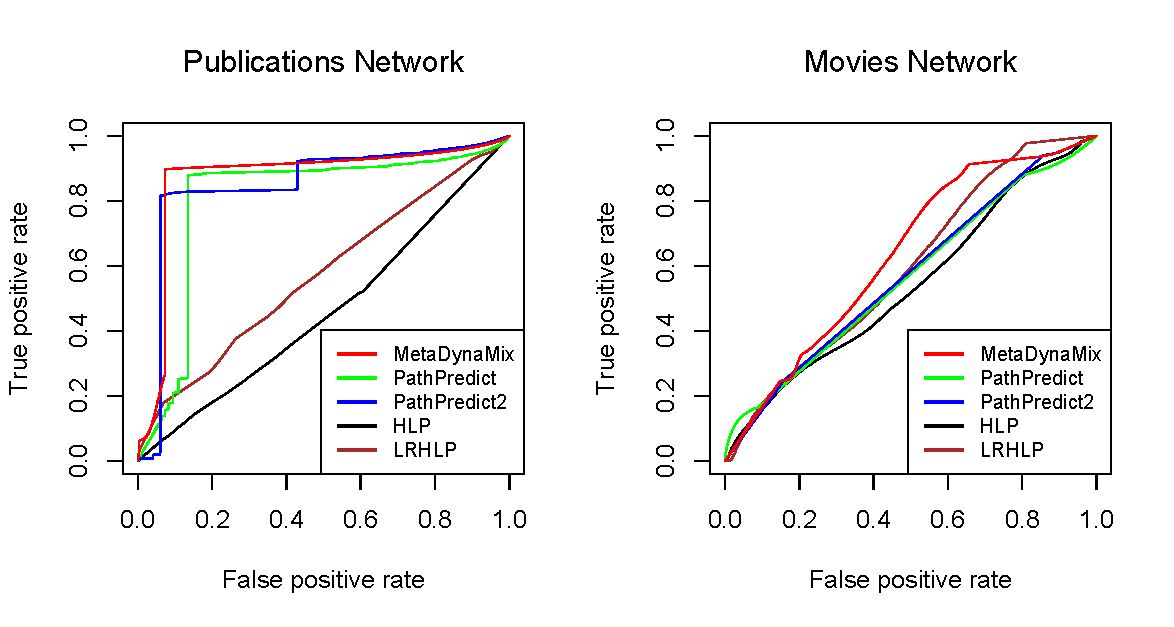
\includegraphics[trim = 0mm 10mm 0mm 0mm,width=0.86\textwidth]{figs/ROC.pdf}
\caption{The ROC curves for different methods and datasets.} \label{fig:auc}
\end{figure}


%\begin{figure}[t]
%\centering
%\subfigure[Publications Network]{
%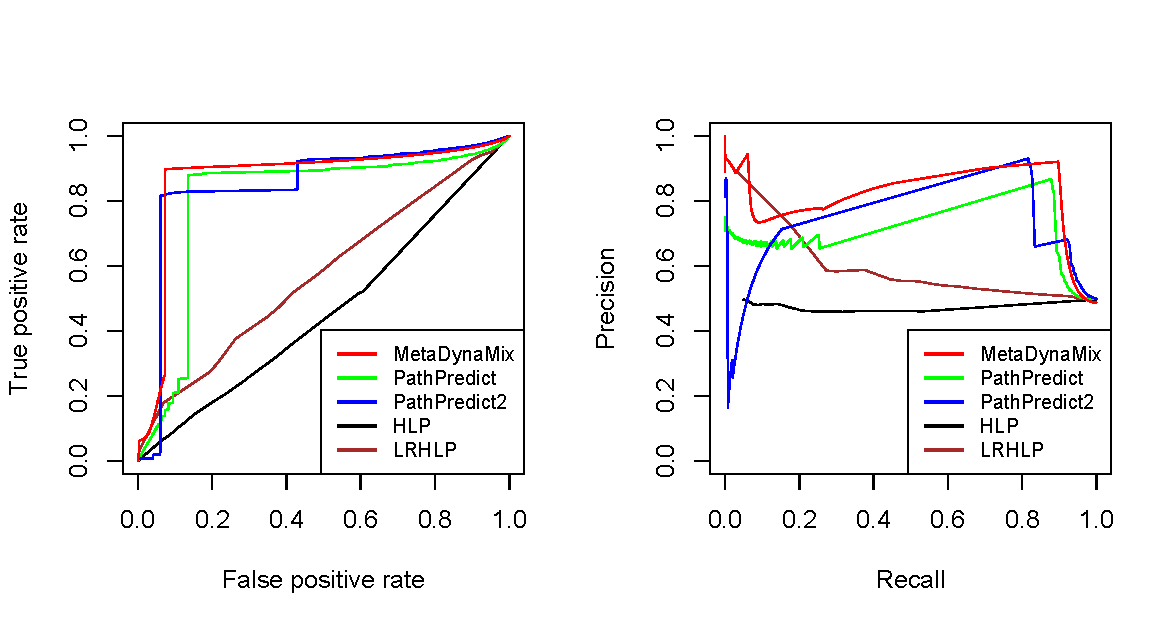
\includegraphics[trim = 0mm 3mm 0mm 0mm,width=0.8\hsize]{figs/DBLP_AUC.pdf}
% \label{Fig:DBLP2}
%}
%\subfigure[Movies Network]{
%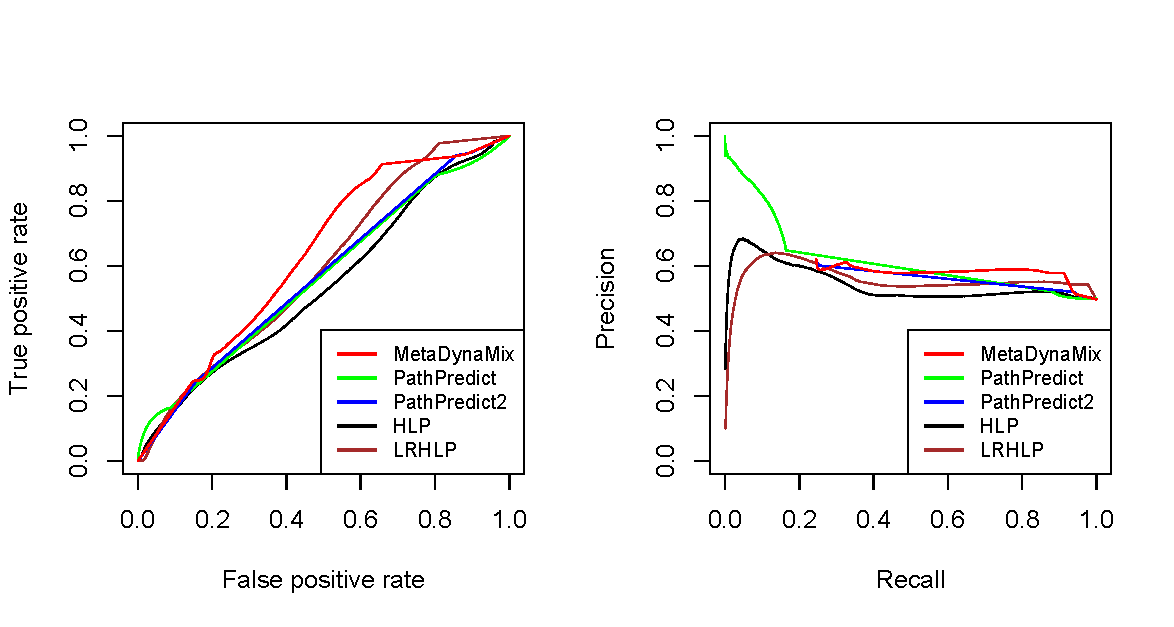
\includegraphics[trim = 0mm 3mm 0mm 10mm,width=0.8\hsize]{figs/IMDB_AUC.pdf}
% \label{Fig:IMDB}
%}
%\caption{The ROC curves for different methods and datasets.} \label{fig:auc}
%\end{figure}


\begin{table}[t]
\centering
\caption{Relationship prediction accuracy comparison. Bold values are determined to be statistically significant compared to the baselines based on McNemar's test.}
\label{table_publications}\label{tbl:auc}
\begin{tabular}{ll|p{1cm}|p{1cm}|p{1cm}||p{1cm}|p{1cm}|p{1cm}|}
\cline{3-8}
                        &   & \multicolumn{3}{l||}{Publications Network} & \multicolumn{3}{l|}{Movies Network} \\ \hline
\multicolumn{1}{|l|}{\textbf{Method}} & \textbf{Metric} & $t$=3 & $t$=5  & $t$=7  & $t$=3  & $t$=5  & $t$=7     \\ \hline\hline

\multicolumn{1}{|l|}{\multirow{2}{*}{PathPredict}}  & ROC  & 0.78 & -- & -- & 0.56 & -- & -- \\ \cline{2-8}
%\multicolumn{1}{|l|}{}  & PR  & 0.45 & -- & -- & 0.45 & -- & -- \\ \cline{2-8}
\multicolumn{1}{|l|}{}  & ACC  & 0.55 & -- & -- & 0.54  & -- & -- \\ \hline\hline

\multicolumn{1}{|l|}{\multirow{2}{*}{PathPredict+}}  & ROC  &  0.78  &   0.80    &     0.83    &   0.56   &    0.57     &    0.57     \\ \cline{2-8}
%\multicolumn{1}{|l|}{}  & PR  &   0.45  &    0.45    &   0.45   &   0.45  &     0.45    &     0.46    \\ \cline{2-8}
\multicolumn{1}{|l|}{}  & ACC  & 0.55  & 0.58  &  0.60 & 0.54  &  0.54  & 0.55   \\ \hline\hline

\multicolumn{1}{|l|}{\multirow{2}{*}{HLP}}  & ROC  &   0.42  &   0.43   &   0.46     &     0.51    &    0.53     &    0.54     \\ \cline{2-8}
%\multicolumn{1}{|l|}{}  & PR  &    0.43  &   0.44   &   0.45    &   0.44   &  0.45   &  0.45  \\ \cline{2-8}
\multicolumn{1}{|l|}{}  & ACC  & 0.50  &  0.50  &  0.50 &  0.51  &  0.52  &  0.53  \\ \hline\hline

\multicolumn{1}{|l|}{\multirow{2}{*}{LRHLP}}  & ROC  &   0.49   &   0.50   &   0.52    &    0.52     &   0.56   &   0.59      \\ \cline{2-8}
%\multicolumn{1}{|l|}{}  & PR  &  0.45    &   0.45   &   0.45   &  0.45   &   0.45   &   0.45      \\ \cline{2-8}
\multicolumn{1}{|l|}{}  & ACC  & 0.47 & 0.50  & 0.51   & 0.52  & 0.56  &  0.58  \\ \hline\hline

\multicolumn{1}{|l|}{\multirow{2}{*}{MetaDynaMix}}  & ROC  & 0.85 &  0.87 & \textbf{0.87}   &  0.57  & 0.59 &  \textbf{0.63}  \\ \cline{2-8}
%\multicolumn{1}{|l|}{}  & PR  & 0.46 &  0.46  &  \textbf{0.46}  &  0.46 &  0.46  & \textbf{0.47}   \\ \cline{2-8}
\multicolumn{1}{|l|}{}  & ACC  & 0.78 & 0.80 & \textbf{0.82}   & 0.56  &  0.60  &   \textbf{0.62} \\ \hline

\end{tabular}
\end{table}


%percentage
%91: our acc for min5 at t=7
%60: pathpred2 acc for min5 at t=7
%50: LRHLP



\textit{Significance of Performance Improvement}. McNemar's test, also called within-subjects $\chi^2$ test, is used to compare statistically significant difference between the accuracy of two predictive models based on the contingency table of their predictions. The null hypothesis indicates that the performances of the two models are equal. We compare MetaDynaMix with the other four baselines and the test results show a $p$-value $<$ 0.0001 for all cases and hence we reject the null hypothesis.

%DBLP
%    179,607 authors had no co-author in 1996-2016. 
%    78,635 authors had no co-author (about 4\%). 
%    ------------
%    100,972 (those who published in 1930-1996)?
%    
%    1,752,443 (total) - 100,972 = 1,651,471 (those who published in 1996-2016)?
%    
%    1,544,408 authors had no co-author in 1930-1996
%    78,635 authors had no co-author (about 4\%). 
%    ------------
%    1,465,773 (those who published in 1996-2016)?
%
%    1,752,443 (total) -1,465,773 = 300,000 (those who published in between)?
    
%    1,752,443 author_papervenuelist_map
%    2,811,533 paper_authorslist_map
%    10,163 venue_paperauthorslist_map
    
%78,635 authors had no co-author (about 4\%)


\textit{The Effect of Time Intervals}. We set the number of time intervals $t$ to 3, 5, and 7 and assess its impact on prediction performance. As presented in Table \ref{tbl:auc}, accuracy increases with the number of snapshots. The intuition is that shorter time interval results in less changes in the graph and thus leads to more reliable predictions. For example considering a meta path \textit{A--P--V--P--A}, with smaller number of intervals, i.e., longer time intervals, we have more distinct authors who have published in a venue in different years and thus more similar path count values. However, by considering more intervals fewer authors will have such relations and more diverse path counts can contribute to more accurate prediction for the next time interval.


%\textit{The Effect of Dimensionality}. For this experiment we only compare prediction performance of MetaDynaMix with $t$=7 on the Publications dataset with respect to different values of $k$. Our results show that for $k$=5, 10, and 20, we get AUCROC values A, B, and 0.87, and ACC values C, D, and 0.82, respectively.\amin{todo: update A,B,C, and D.}

\section{Related Work}

\cite{Zhu2016} \cite{sun2011pathsim} \cite{Sun:2012:HRP:2124295.2124373} \cite{huang2016meta}
\cite{wang2016relsim} \cite{sun2013pathselclus} \cite{sun2011ASONAM} \cite{Yang2012} \cite{liben2007link}


Matrix factorization technique \cite{menon2011link} has been used for link prediction... the effectiveness of the structural link prediction problem, inspired by their success in collaborative filtering... as learning latent features from the data, and why it can be expected to be more predictive than popular unsupervised scores. 

Such methods are homogeneous and non-temporal. The number of common neighbors \cite{newman2001clustering}, preferential attachment \cite{newman2001clustering}, Jaccard's coefficient \cite{liben2007link}, and Katz$\beta$ \cite{katz1953new}, are amongst frequently used topological features defined in homogeneous networks.


Sun et al. proposed PathSelClus \cite{sun2013pathselclus} that uses limited guidance from users in the form of seeds in some of the clusters and automatically learn the best weights for each meta-path in the clustering process.

The concept of temporal smoothness has been used in evolutionary clustering [36] and link prediction in a dynamic network \cite{Zhu2016}.

While many graph embedding methods exist for static networks, few considered dynamic networks. Zhu et al. \cite{Zhu2016} attempt dynamic link prediction by adding a temporal-smoothing regularization term to a non-negative matrix factorization objective. They use a block-coordinate gradient descent algorithm to perform non-negative factorization. Their formulation is almost identical to the algorithm of Chi et al. \cite{Chi:2007}, who perform evolutionary spectral clustering that captures temporal smoothness. Because matrix factorization provides embedding vectors of the nodes for each time-stamp, the factorization by-product from this work can be considered as dynamic network embeddings.



% Link prediction is pervasive in biological network analysis, where verifying the existence of links between nodes requires costly experimental tests. Limiting the experiments to links ordered by presence likelihood has been shown to be very cost effective. In social networks, link prediction is used to predict probable friendships, which can be used for recommendation and lead to a more satisfactory user experience. Liben-Nowell et al. \cite{liben2007link}, Lu et al. [52] and Hasan et al. [53] survey the recent progress in this field and categorize the algorithms into (a) similarity based (local and global) [13], [14], [54], (b) maximum likelihood based [15], [16] and (c) probabilistic methods [17], [18], [55]. 
%Embeddings capture inherent dynamics of the network either explicitly or implicitly thus enabling application to link prediction. Wang et al. [23] and Ou et al. [24] predict links from the learned node representations on publicly available collaboration and social networks. In addition, Grover et al. [29] apply it to biology networks. They show that on these data sets links predicted using embeddings are more accurate than traditional similarity based link prediction methods described above.


% [13] P. Jaccard, Etude comparative de la distribution florale dans une portion des Alpes et du Jura. Impr. Corbaz, 1901.
% [14] L. A. Adamic and E. Adar, “Friends and neighbors on the web,” Social networks, vol. 25, no. 3, pp. 211–230, 2003.
% [15] A. Clauset, C. Moore, and M. E. Newman, “Hierarchical structure and the prediction of missing links in networks,” Nature, vol. 453,
% no. 7191, pp. 98–101, 2008.
% [16] H. C. White, S. A. Boorman, and R. L. Breiger, “Social structure from multiple networks. i. blockmodels of roles and positions,” American journal of sociology, vol. 81, no. 4, pp. 730–780, 1976.
% [17] N. Friedman, L. Getoor, D. Koller, and A. Pfeffer, “Learning probabilistic relational models,” in IJCAI, 1999, pp. 1300–1309.
% [18] D. Heckerman, C. Meek, and D. Koller, “Probabilistic entityrelationship models, prms, and plate models,” Introduction to statistical relational learning, pp. 201–238, 2007.
% [23] D. Wang, P. Cui, and W. Zhu, “Structural deep network embedding,” in Proceedings of the 22nd International Conference on Knowledge Discovery and Data Mining. ACM, 2016, pp. 1225–1234.
% [24] M. Ou, P. Cui, J. Pei, Z. Zhang, and W. Zhu, “Asymmetric transitivity preserving graph embedding,” in Proc. of ACM SIGKDD, 2016, pp. 1105–1114.
% [29] A. Grover and J. Leskovec, “node2vec: Scalable feature learning for networks,” in Proceedings of the 22nd International Conference on Knowledge Discovery and Data Mining. ACM, 2016, pp. 855–864.
% [52] L. Lu and T. Zhou, “Link prediction in complex networks: A survey,” Physica A: Statistical Mechanics and its Applications, vol.
% 390, no. 6, pp. 1150–1170, 2011.
% [53] M. Al Hasan and M. J. Zaki, “A survey of link prediction in social networks,” in Social network data analytics, 2011, pp. 243–275.
% [54] L. Katz, “A new status index derived from sociometric analysis,”
% Psychometrika, vol. 18, no. 1, pp. 39–43, 1953.
% [55] K. Yu, W. Chu, S. Yu, V. Tresp, and Z. Xu, “Stochastic relational models for discriminative link prediction,” in NIPS, 2006, pp. 1553–1560.
\section{Conclusions and Future Work}

We studied the problem of relationship prediction in DHINs and proposed a supervised learning framework based on a combined set of latent and topological meta path-based features. Our results show that the proposed technique significantly improves prediction accuracy compared to the baseline methods. In this work we did not evaluate the running time and efficiency of our approach. Since our major computational bottleneck is calculating meta path-based measures, such as path count, we would like to investigate approximation techniques to make the prediction scalable. Furthermore we are interested in enhancing the matrix factorization technique based on a loss function that does not require full topological features matrix. In addition to model improvement, another interesting direction is to investigate the effectiveness of our proposed approach in other applications, such as predicting interests of users in a social media, that can be formulated as a link/relationship prediction problem.


\bibliographystyle{ACM-Reference-Format}
\bibliography{refs}

\end{document}
